\documentclass[a4paper, twoside,openright]{report}

% Dimensione dei margini
\usepackage[a4paper,top=3cm,bottom=3cm,left=3cm,right=3cm]{geometry} 
% Dimensione del font
\usepackage[fontsize=12pt]{scrextend}
% Lingua del testo
\usepackage[english,italian]{babel}
% Lingua per la bibliografia
\usepackage[fixlanguage]{babelbib}
% Codifica del testo
\usepackage[utf8]{inputenc} 
% Encoding del testo
\usepackage[T1]{fontenc}
% Permette di generare testo fittizio. Mi è stato utile 
% per capire quale sarebbe stata l'impostazione del 
% testo nella pagina prima che scrivessi un determinato paragrafo
\usepackage{lipsum}
% Per ruotare le immagini
\usepackage{rotating}
% Per modificare l'header delle pagine 
\usepackage{fancyhdr}               

% Librerie matematiche
\usepackage{amssymb}
\usepackage{amsmath}
\usepackage{amsthm}         

% Uso delle immagini
\usepackage{graphicx}
% Uso dei colori
\usepackage[dvipsnames]{xcolor}         
% Uso dei listing per il codice
\usepackage{listings}          
% Per inserire gli hyperlinks tra i vari elementi del testo 
\usepackage{hyperref}     
% Diversi tipi di sottolineature
\usepackage[normalem]{ulem}

% -----------------------------------------------------------------

% Modifica lo stile dell'header
\pagestyle{fancy}
\fancyhf{}
\lhead{\rightmark}
\rhead{\textbf{\thepage}}
\fancyfoot{}
% \setlength{\headheight}{12.5pt}
\setlength{\headheight}{15.6pt}

% Rimuove il numero di pagina all'inizio dei capitoli
\fancypagestyle{plain}{
  \fancyfoot{}
  \fancyhead{}
  \renewcommand{\headrulewidth}{0pt}
}

% Stile del codice
\lstdefinestyle{codeStyle}{
    % Colore dei commenti
    commentstyle=\color{teal},
    % Colore delle keyword
    keywordstyle=\color{Magenta},
    % Stile dei numeri di riga
    numberstyle=\tiny\color{gray},
    % Colore delle stringhe
    stringstyle=\color{violet},
    % Dimensione e stile del testo
    basicstyle=\ttfamily\footnotesize,
    % newline solo ai whitespaces
    breakatwhitespace=false,     
    % newline si/no
    breaklines=true,                 
    % Posizione della caption, top/bottom 
    captionpos=b,                    
    % Mantiene gli spazi nel codice, utile per l'indentazione
    keepspaces=true,                 
    % Dove visualizzare i numeri di linea
    numbers=left,                    
    % Distanza tra i numeri di linea
    numbersep=5pt,                  
    % Mostra gli spazi bianchi o meno
    showspaces=false,                
    % Mostra gli spazi bianchi nelle stringhe
    showstringspaces=false,
    % Mostra i tab
    showtabs=false,
    % Dimensione dei tab
    tabsize=2
} \lstset{style=codeStyle}

% Stile di codice per dimensioni maggiori, in cui ho avuto bisogno di un testo più picolo (ad esempio se si vuole inserire del codice che ha linee molto lunghe). Per usare questo stile piuttosto che il precedente, usare 

% \lstset{style=longBlock}
%  % inserire il codice...
% \lstset{style=codeStyle}

% Il secondo comando consente di tornare allo stile precedente 
\lstdefinestyle{longBlock}{
    commentstyle=\color{teal},
    keywordstyle=\color{Magenta},
    numberstyle=\tiny\color{gray},
    stringstyle=\color{violet},
    basicstyle=\ttfamily\scriptsize,
    breakatwhitespace=false,         
    breaklines=true,                 
    captionpos=b,                    
    keepspaces=true,                 
    numbers=left,                    
    numbersep=5pt,                  
    showspaces=false,                
    showstringspaces=false,
    showtabs=false,                  
    tabsize=2
} \lstset{style=codeStyle}

% Togliendo il commento al comando che segue, si inseriscono nella bibliografia anche le fonti presenti in Bibliography.bib ma non citati direttamente con il comando \cite
% \nocite{*}

% Margini prima e dopo blocchi di codice, per avere più distanza
\lstset{aboveskip=20pt,belowskip=20pt}

% Modifica dello stile dei riferimenti, con il testo in cyano
\hypersetup{
    colorlinks,
    linkcolor=CornflowerBlue,
    citecolor=CornflowerBlue
}

% Aggiunti definizioni, teoremi, linea e listing
\newtheorem{definition}{Definizione}[section]
\newtheorem{theorem}{Teorema}[section]
\providecommand*\definitionautorefname{Definizione}
\providecommand*\theoremautorefname{Teorema}
\providecommand*{\listingautorefname}{Listing}
\providecommand*\lstnumberautorefname{Linea}

\raggedbottom

%\newcommand{\cgs}[1]{{\textcolor{brown}[\textcolor{red}{\bf{GS: }}{ \textcolor{brown}{#1]}}}}             
%\newcommand{\cmc}[1]{{\textcolor{blue}[\textcolor{magenta}{\bf{MC: }}{ \textcolor{blue}{#1]}}}}


% SIMONE
\usepackage{xcolor}
\newcommand{\highlighttext}[1]{\texttt{\color[HTML]{BB5500} #1}}
% SIMONE


% -----------------------------------------------------------------
\begin{document}

% \begin{titlepage}
\begin{figure}[!htb]
    \centering
    
\includegraphics[keepaspectratio=true,scale=0.5]{images/Frontespizio/cherubinFrontespizio.eps}
\end{figure}

\begin{center}
    \LARGE{UNIVERSITÀ DI PISA}
    \vspace{5mm}
    \\ \large{DIPARTIMENTO DI INGEGNERIA DELL'INFORMAZIONE}
    \vspace{5mm}
    \\ \LARGE{Laurea Triennale in Ingegneria Informatica}
\end{center}

\vspace{15mm}
\begin{center}
    {\LARGE{\bf Un fantastico titolo\\ \vspace{5mm} per la mia tesi di laurea! }}
    
    % Se il titolo è abbastanza corto da stare su una riga, si può usare
    
    % {\LARGE{\bf Un fantastico titolo per la mia tesi!}}
\end{center}
\vspace{30mm}

\begin{minipage}[t]{0.47\textwidth}
	{\large{Relatore:}{\normalsize\vspace{3mm}
	\bf\\ \large{Prof: Nome Cognome} \normalsize\vspace{3mm}\bf \\ \large{Prof: Nome Cognome}}}
\end{minipage}
\hfill
\begin{minipage}[t]{0.47\textwidth}\raggedleft
	{\large{Candidato:}{\normalsize\vspace{3mm} \bf\\ \large{Nome Cognome}}}
\end{minipage}

\vspace{30mm}
\hrulefill
\\\centering{\large{ANNO ACCADEMICO 202X/202Y}}

\end{titlepage}
% \include{chapters/Abstract}

\tableofcontents

% Rimuovere se non si vuole la tabella delle figure
\listoffigures

\cite{LabelPerLaCitazione}
\chapter{Classification}

In this task, our goal was to create a classifier which, given an incident, would predict the presence of a fatality. 

Two different classifiers have been tested: a Decision Tree, for it's interpretable nature, and a Neural Network, for it's ability to capture complex relationships between the features.

\section{Methods}

Since the target variable comes from the dataset in the form of \highlighttext{n\_killed} which is the number of fatalities, it was necessary to transform it into a binary variable (\highlighttext{isKilled}) and to drop the original one and all the features directly derivating from it.

\subsection{Feature Selection}

Some early tests showed nearly perferct results from the classifiers. Analyzing the Decision Tree it was easy to see that the classifier was obtaining the value of \highlighttext{n\_killed} from \highlighttext{n\_participants - n\_injured - n\_unharmed - n\_arrested}.

To avoid this problem, \highlighttext{n\_participants} and all the features that would allow to obtain it were dropped.

Later tests showed that the classifier was still \textit{cheating} when \highlighttext{n\_injured} == \highlighttext{n\_unharmed} == \highlighttext{n\_arrested} == 0; in this case, given that \highlighttext{n\_participants} $\geq 1$, the value of \highlighttext{n\_killed} would be $\geq 1$. To avoid artificially inflating the scores, the datapoints where this condition was met were dropped. 

\subsection{Scaling}

For the Decision Tree classifier, no scaling was necessary, so it was not performed to keep the interpretability of the model.

For the Neural Network, the dataset was scaled using the \highlighttext{StandardScaler} from SKLearn.

\subsection{Training-Validation-Test split}

The dataset was split into three parts: training ($70\%$), validation ($15\%$) and test ($15\%$). The training set was used to train the classifier, the validation set was used evaluate the difference in performance between different classifiers and to tune the hyperparameters, and the test set was used to evaluate the final performance of the classifiers.

\subsection{Balancing}

The dataset is unbalanced, with around $75\%$ of incidents having no fatalities. This could lead to a classifier that always predicts no fatalities. To avoid this problem the dataset was balanced using the \highlighttext{SMOTE}\cite{chawla2002smote} algorithm on the training set, and with upsampling with replacement on the validation and test sets (to avoid testing on syntetic data).


\section{Decision Tree}

SKLearn's Decision Tree classifier was used. To try to avoid overfitting, a Grid Search was performed.

Despite this, the best classifier obtained had an F1 score of $0.93$ on the training set, while on the validation set it had an F1 score of $0.72$.

\begin{figure}[h]
    \centering
    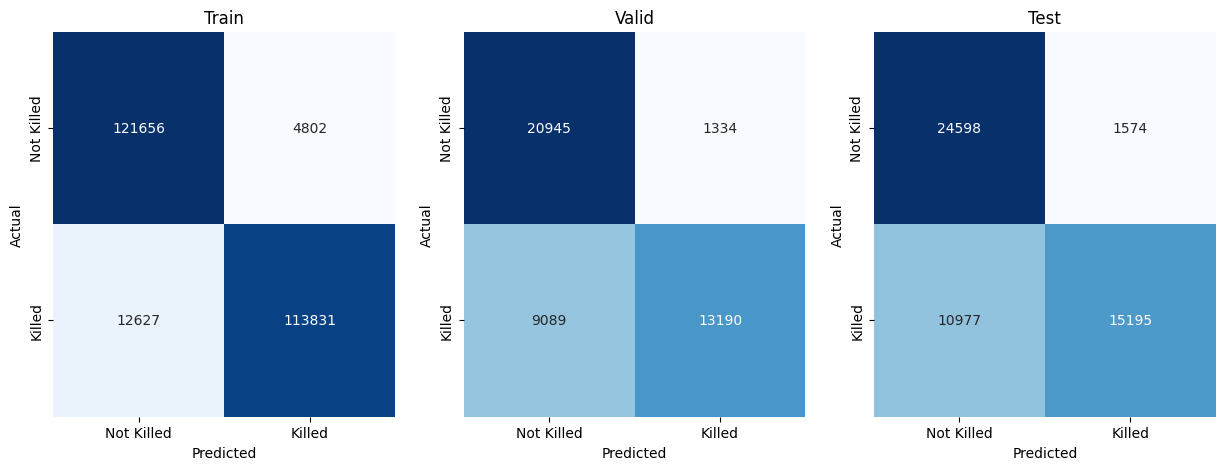
\includegraphics[width=\textwidth]{images/Clustering/decision_tree_cm.png}
    \caption{Decision Tree confusion matrix of the training, validation and test sets.}
    \label{fig:decision_tree_cm}
\end{figure}

On Figure \ref{fig:decision_tree_cm} the confusion matices of the training, validation and test sets can be analyzed. While still having positive results, the classifier is clearly overfitting.

The final test F1 score was $0.71$. Figure \ref{fig:decision_tree} shows the first three levels of the Decision Tree.

\begin{figure}[h]
    \centering
    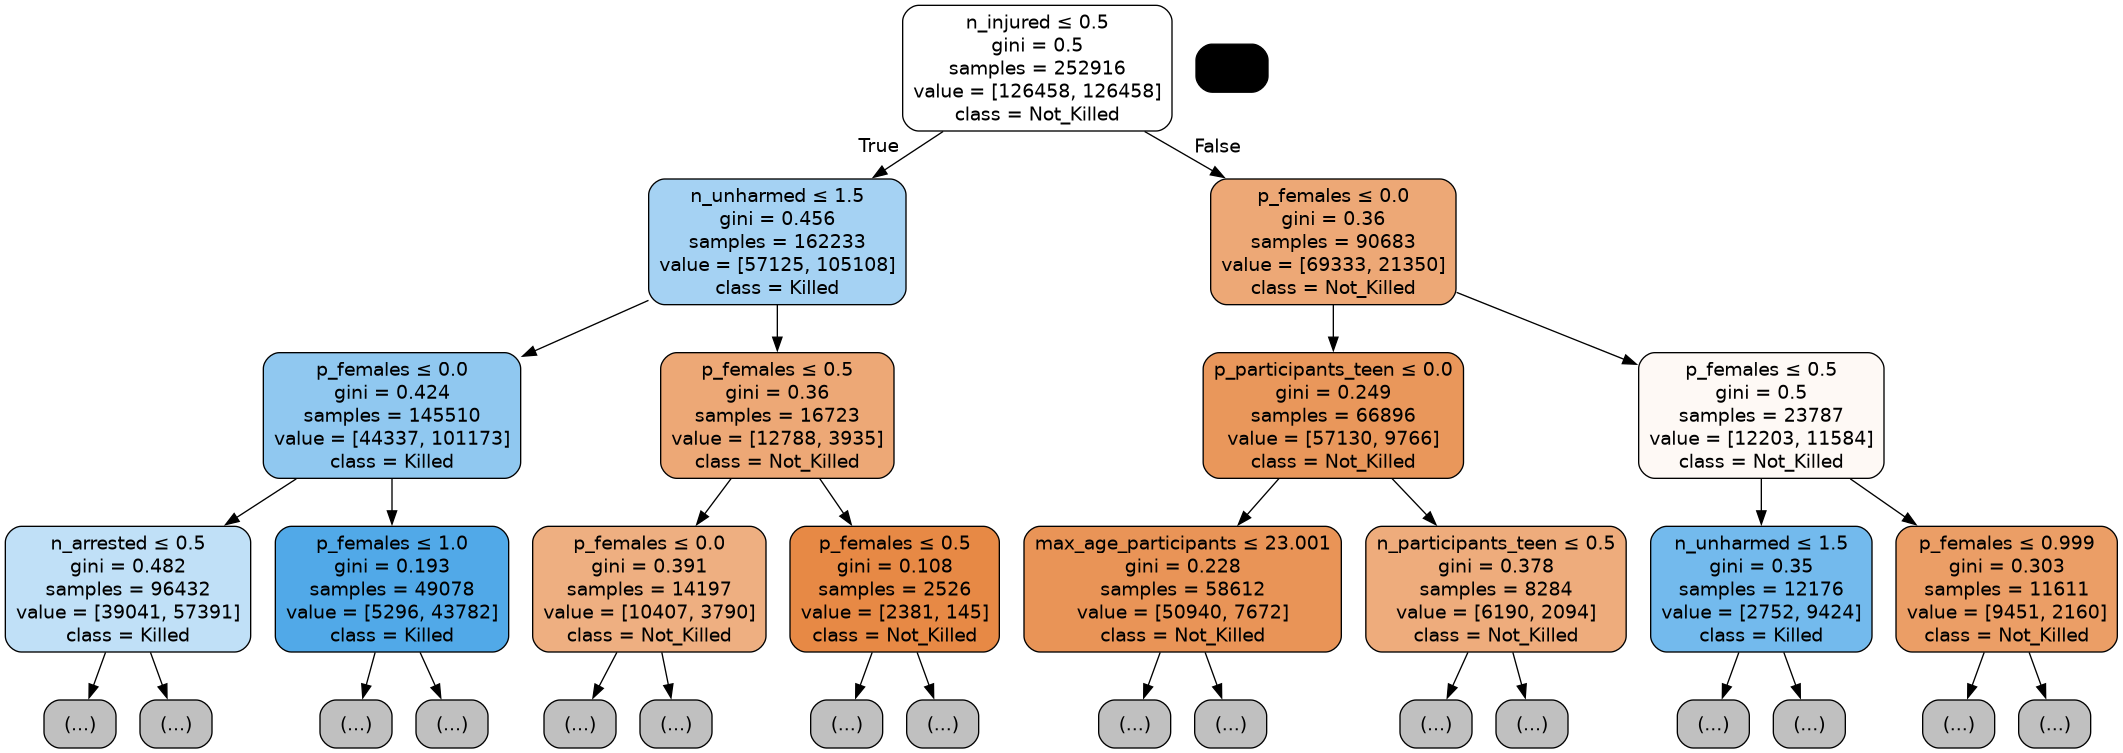
\includegraphics[width=\textwidth]{images/Clustering/decision_tree.png}
    \caption{Decision Tree.}
    \label{fig:decision_tree}
\end{figure}

\section{Neural Network}

A Neural Network was trained hoping that it would find hidden relations in the data. The architecture used was the following:

\begin{itemize}
    \item Input layer with 23 neurons (one for each feature)
    \item 4 Hidden layers with [32, 16, 8, 4] neurons and Sigmoid activation function, followed by a 10\% dropout rate
    \item Output layer with 2 neurons and Softmax activation function
\end{itemize}

The model was trained with an Early Stopping callback, which stopped the training if the validation score did not improve for 10 validation steps.

The Early Stopping kicked in at the 13000th epoch, with a training F1 score of $0.82$ and a validation F1 score of $0.78$.

\begin{figure}[h]
    \centering
    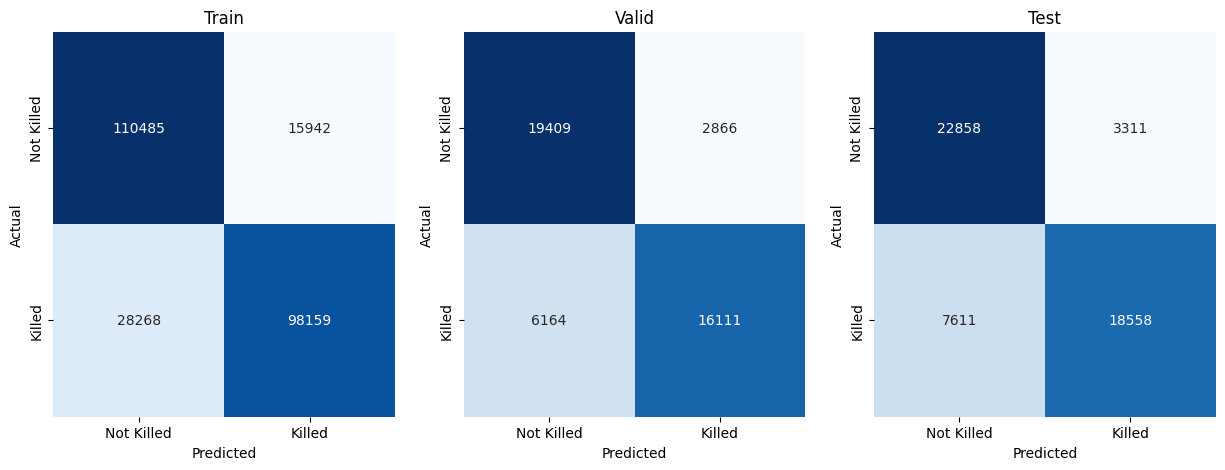
\includegraphics[width=\textwidth]{images/Clustering/nn_cm.png}
    \caption{Neural Network confusion matrix of the training, validation and test sets.}
    \label{fig:nn_cm}
\end{figure}

Figure \ref{fig:nn_cm} shows the confusion matrices of the training, validation and test sets. The final test F1 score was $0.77$. 

\section{Comparison}

\begin{figure}[h]
    \centering
    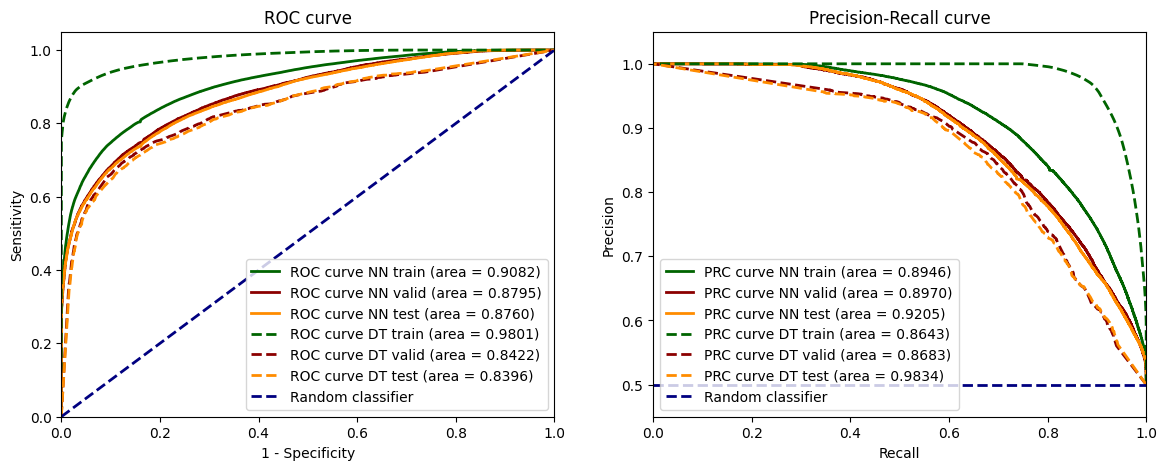
\includegraphics[width=\textwidth]{images/Clustering/roc-prc.png}
    \caption{ROC and Precision-Recall curves of the Decision Tree and Neural Network compared.}
    \label{fig:roc}
\end{figure}

Figure \ref{fig:roc} shows the ROC and Precision-Recall curves of the Decision Tree and Neural Network compared. 

The Neural Network has a slight advantage over the Decision Tree, with higher scores on the test set, but not significat enough to mark it as better suited for the task.

\begin{quotation}
    \small
    It is important to note that due to hardware limitations, the search for the best hyperparameters was not exhaustive, and it is possible that better results could be obtained with a more thorough search.
\end{quotation}
% \chapter{Timeseries Analysis}


\section{Dataset Preparation}

To start our analysis we needed to once again prepare the dataset.
We started by working on the $final clean 3$ dataset by only keeping the incidents between 2014 and 2017 and by adding to each incident the week in which it took place.
Finally we created a dataframe called $clean city df$ in which we kept only the cities with a number of incidents greater than the 15$\%$ of incidents in the 209 weeks total.

\section{City Score}

For the first analysis on the motifs and anomalies we decided for a score that incorporated the number of killed people in each incident.
This score for each city is defines as follows:
\textit{Score $=$ number of killed people in that week + number of injured people in that week $* 0.8 +$ number of arrested people in that week $* 0.5 +$  number of child participants in that week $+$ number of teen participants in that week $* 0.8 +$ number of adult participants in that week $* 0.5$}
It can be considered as a positive weighted sum where the weights are chosen arbitrarily and can be changed based on the importance that we want to give to each indicator.
we gave a higher weight to the number of killed and injured people, and a lower weight to the number of arrested people
We also gave a higher weight to the number of children and teenagers involved in the incident, and a lower weight to the number of adults involved
Defined in this way the score can be interpreted as a measure of the severity of each incident.

\begin{figure}[ht]
    \centering
    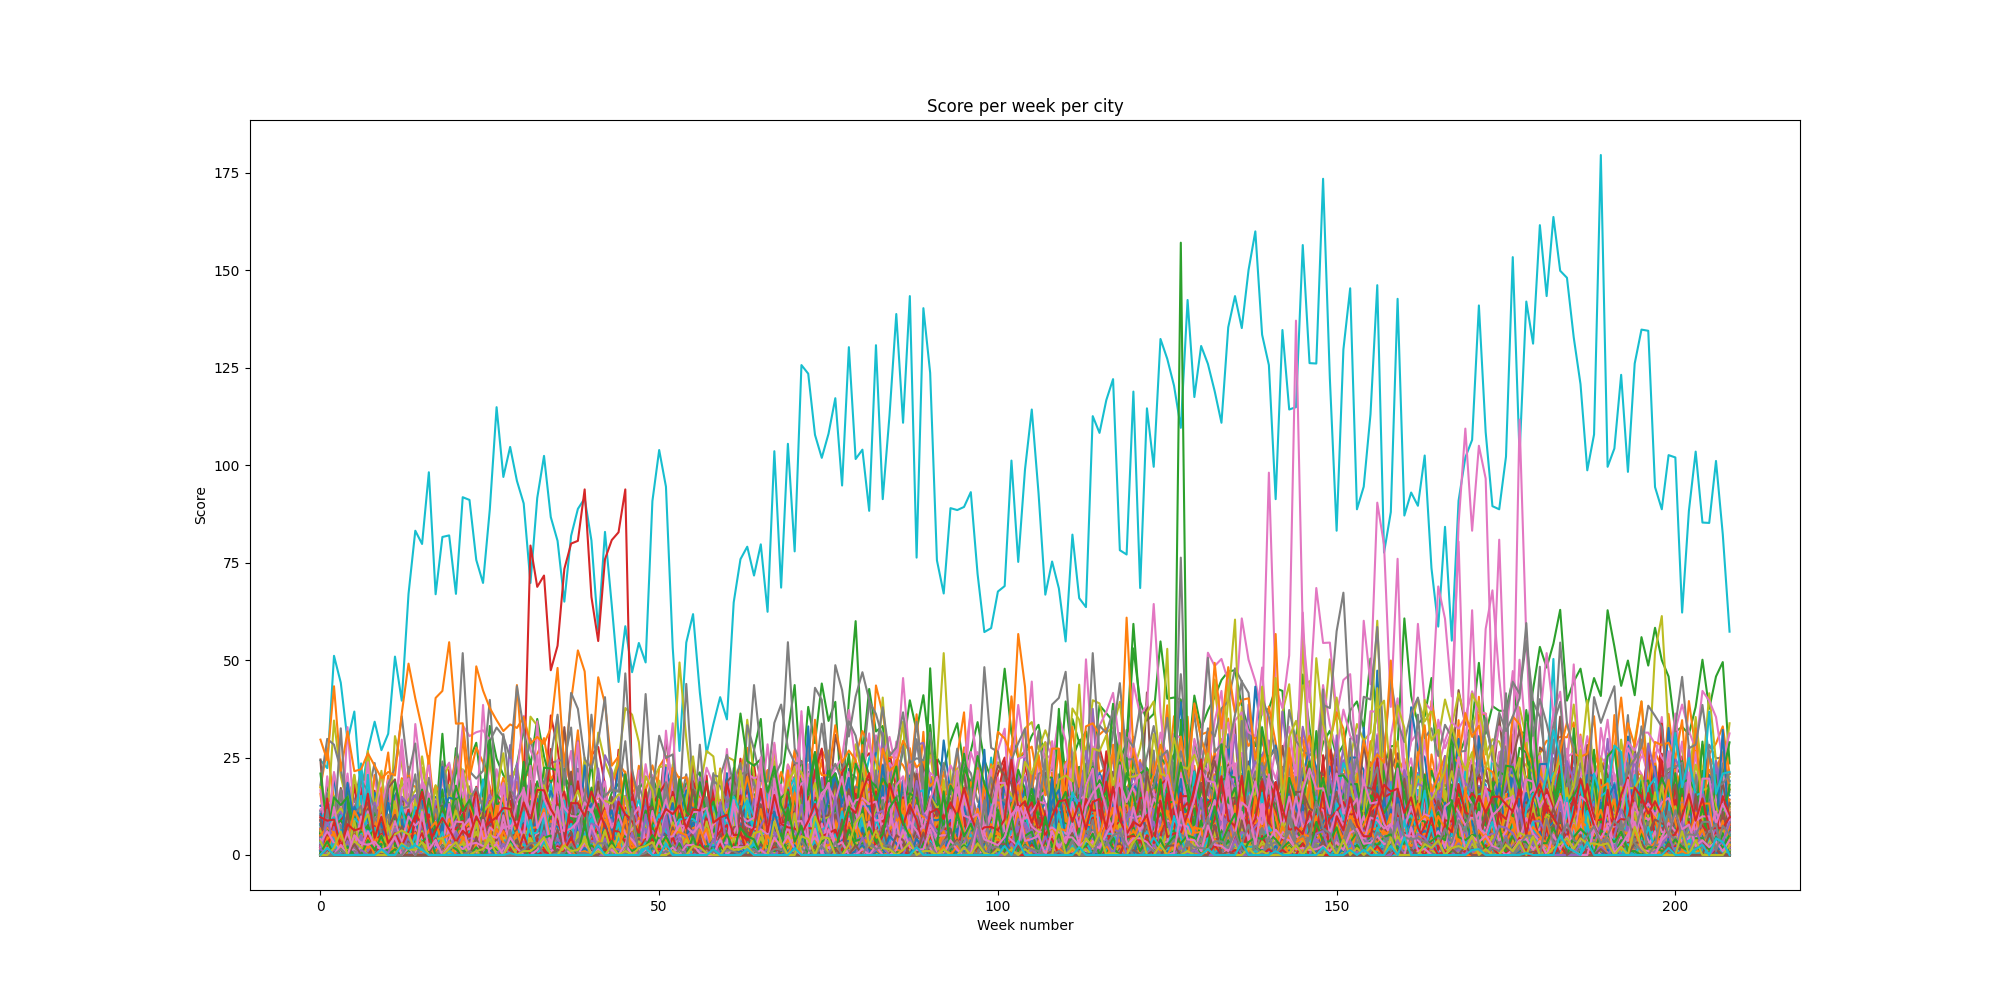
\includegraphics[width= 0.8\textwidth]{images/Capitolo1/score_per_week_per_city.png} 
    \caption{Questa è un'immagine} 
    \label{fig:score_per_week_per_city}
\end{figure}

\subsection{Scaled Timeseries}

We decided to also test the clustering on the timeseries scaled with the standard scaler and the minmax scaler, to see if doing so would result in better clusters

In the following figure we can see the plot for all the timeseries scaled in this way

\begin{figure}[ht]
    \centering
    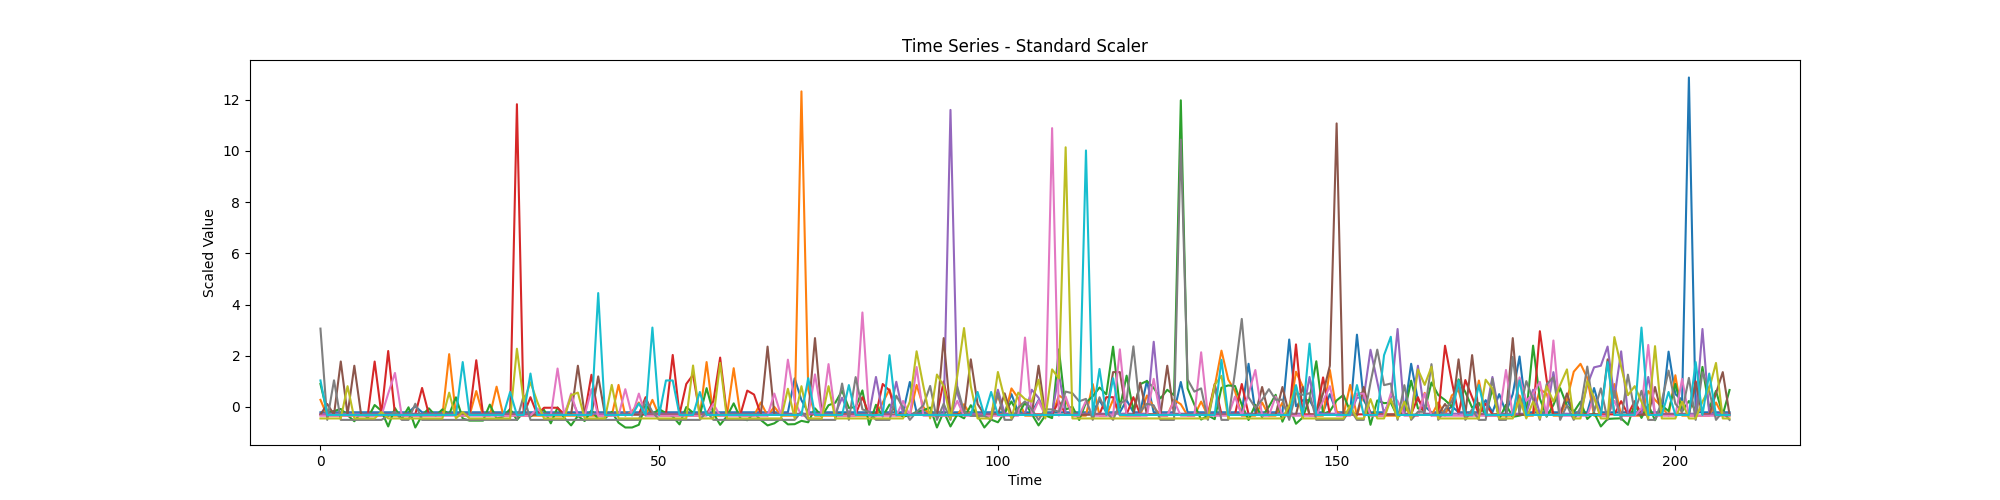
\includegraphics[width= 0.8\textwidth]{images/Capitolo1/time_series_standard_scaler.png} 
    \caption{Questa è un'immagine} 
    \label{fig:time_series_standard_scaler}
\end{figure}

\begin{figure}[ht]
    \centering
    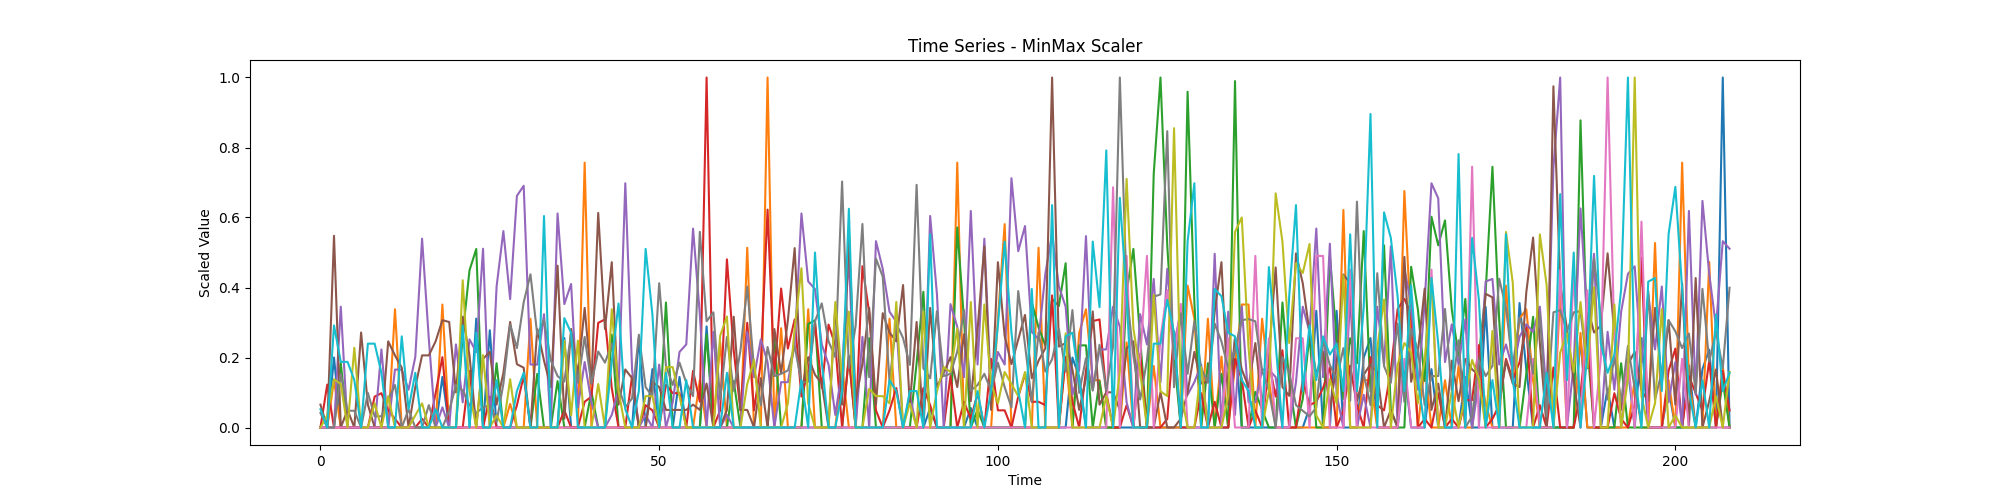
\includegraphics[width= 0.8\textwidth]{images/Capitolo1/time_series_minmax_scaler.png} 
    \caption{Questa è un'immagine} 
    \label{fig:time_series_minmax_scaler}
\end{figure}


\section{Clustering}

For the cluster analysis we decided to not test most of the algorithms because we already tested them in previous section of the project.
So we decided to concentrate on K-means on the raw time series and on their features.
We also skipped the euclidean distance and decided to use the Dynamic Time Warping (DTW) mainly because it is better suited to capture time series with varying pattern, time shifts or speed, all things that euclidean distance could miss.


\subsection{Clustering on the raw Timeseries}

We applied K-means on the original timeseries and also on the one scaled with the standard scaler and the minmax scaler.

To find the best number of cluster we used the same technique that we used in the clustering of the incident dataset, the silhouette score.

As seen in the table, both the standard scaler and the minmax scaler resulted in a significant reduction of the clustering score, while the original timeseries reached a 0.8. 


\subsection{Clustering on the feature of the Timeseries}

Another technique often used when dealing with Timeseries is to reduce each one of them to a vector containing some significant feature of the Timesearies, such as mean, variance, kurtosis ecc..  and then apply the clustering algorithms to those points.

Same as the clustering on raw time series we performed K-means on the initial timeseries, the timeseries scaled with the standard scaler and the one scaled with the minmax scaler.
We registered a significant increase in the silhouette score for all three of the timeseries, a number much greater than the one for the corresponding initial timeseries.
In particular feature clustering on the original timeseries seems to best differentiate the two clusters found





\subsection{Comparison of the clustering with a random walk}

To test how well K-means worked on our timeseries we generated the same number of random walk with the same number of points and with the same min and max value as our standard timeseries.

We then procedeed to use K-means on the standard random timeseries and discovered a silhouette score close to zero, confirming that our time series were clustered better than randomly.
The same conclusion was reached also on the feature based cluster, in which even though the clustering on the random timeseries reached $0.50$ it was still significantly lower than the corresponding score on the original timeseries




\section{Motif and Anomaly Detection}

The timeseries chosen for the motif discovery are the two cluster centroids found with K-means in the previous point.
Altough the significance of those two timeseries could be discussed, the idea behind it is that no timeseries is significant enough to conduct this kind of analysis on.
We should consider them equal and in this way analyze each city one by one.
Because it was not possible to study that many city, we opted to take the two timeseries that describe the two different clusters.
Another possible analysis could be conducted on a small sample from each of those clusters, but still this analysis is not that much more significant.

The only interesting thing that we can notice is the 'absence' of motifs in the random series, which is to be expected, while we can always find some motif in our timeseries, scaled or not scaled.

As far as Anomaly detection, we conducted it on the non scaled Timeseries, and we were able to find a couple of anomalies, but also these anomalies cannot really be interpreted in a nice way.

For comparison, we also took a couple of the cities with the highest score and the one with the lowest and conducte the motif and anomaly discovery on those.

The results were similar to the one on the cluster centers, because nothing particularly interesting emerged, except that the motif alternated between each other.



\section{Shapelets}

For the analysis on the Shapelets of the time series, we needed to create  new indicator.
The new score for each city is defined as follows:
\textit{Score\textunderscore Shapelet $=$ number of incidents in that week + number of participants in incidents in that week}

In this case the main idea behind this score is that by summing the number of incidents and the number of people involved we could get a decent indirect correlation with the given label is\textunderscore killed.

We chose the threshold after which a timeseries would be considered as a positive is\textunderscore killed value, in a way to make the number of positive city almost the same as the negative cities, mainly to make classification more precise.

For the shapelet extraction, due to the high computational cost of the algorithms, decided to take only a small sample of the time series and extract the shapelet from those.
We also tried to use the tensorflow library but gave results that suggested some kind of problem, so we used the alternative method for finding the shapelets (pyts library)

Despite the low number of samples, the F1 score of the classifier got an accuracy of 0.83 and a decent ROC curve





















% \section{Clustering}

\begin{frame}
    \frametitle{Clustering}
    \begin{exampleblock}{Preparation }
        
    
        \begin{itemize}
            \item IQR method for outliers detection
            \item Min-Max scaling
            \item Silhouette score for evaluation
        \end{itemize}
    \end{exampleblock}    
\end{frame}

%%%%%%%%%%%%%%%%%%%%%%%%%%%%%%%%%%%%%%%%%%%%%%%%%%%%%%%%%%%%%%%%%%%%%%%%%%

\begin{frame}
    \frametitle{Clustering}

\begin{exampleblock}{K-Means}
    \begin{itemize}
        \item Entire dataset
        \item Parameter: $k$ (number of clusters)
    \end{itemize}
\end{exampleblock}
\begin{exampleblock}{DBSCAN}
    \begin{itemize}
        \item State: California
        \item Parameters: {
            \begin{itemize}
                \item $\epsilon$ (neighborhood radius)
                \item $n$ (core points neighborhood minimum size)
            \end{itemize}
        }
        
    \end{itemize}
\end{exampleblock}
\begin{exampleblock}{Hierarchical}
    \begin{itemize}
        \item State: California
        \item Parameter: inter-cluster distance
    \end{itemize}
\end{exampleblock}

\end{frame}

%%%%%%%%%%%%%%%%%%%%%%%%%%%%%%%%%%%%%%%%%%%%%%%%%%%%%%%%%%%%%%%%%%%%%%%%%%

\begin{frame}{K-means}
    \begin{exampleblock}{Selected features:}
        \begin{itemize}
            \item state\_population
            \item timestamp
            \item p\_injured
            \item month\_cd\_change\_min\_age\_participants
            \item month\_cd\_ratio\_males
        \end{itemize}        
    \end{exampleblock}


    
    \begin{table}[]
        \centering
        \begin{tabular}{|lc|}
    
            \hline
            \textbf{Clustering}  & C6 \\
            \textbf{K} & 2\\
            \textbf{Clusters sizes} & (59466, 35725) \\
            \textbf{Silhouette mean} & 0.453778 \\
            \textbf{Silhouette variance} & 3.048582e-08 \\
            \hline

        \end{tabular}
        \label{tab:my_label}
    \end{table}
\end{frame}

%%%%%%%%%%%%%%%%%%%%%%%%%%%%%%%%%%%%%%%%%%%%%%%%%%%%%%%%%%%%%%%%%%%%%%%%%%

\begin{frame}{K-means}
    \begin{figure}
        \centering
        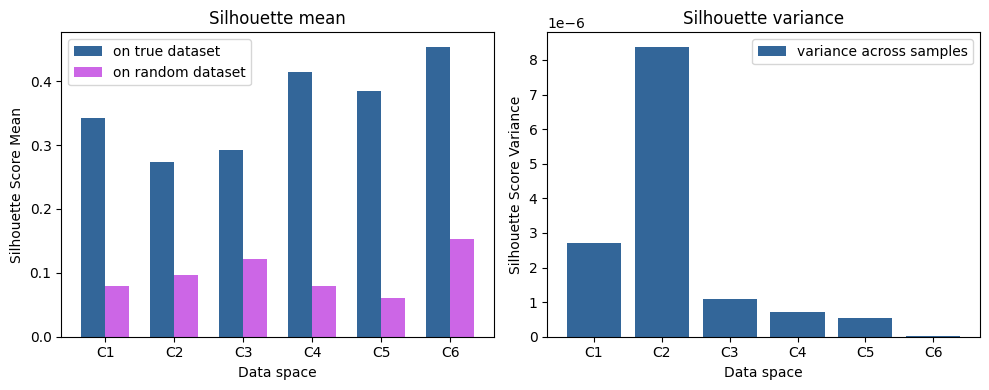
\includegraphics[width=.99\textwidth]{img/clustering/kmeans.png}
        \label{kmeans}
    \end{figure}
\end{frame}


%%%%%%%%%%%%%%%%%%%%%%%%%%%%%%%%%%%%%%%%%%%%%%%%%%%%%%%%%%%%%%%%%%%%%%%%%%

\begin{frame}{DBSCAN}

    \begin{exampleblock}{Selected features:}
        \begin{itemize}
            \item latitude
            \item min\_age\_participants
            \item n\_killed
        \end{itemize}
           
    \end{exampleblock}
    
    \begin{table}[]
        \centering
        \begin{tabular}{|lc|}
            \hline
              \textbf{Clustering}  & C4 \\
              $\epsilon$  & 0.6 \\
              $n$ & 21 \\
              \textbf{K} & 2\\
              \textbf{Clusters sizes} & (2088, 3938) \\
              \textbf{Silhouette} & 0.670266 \\
              \hline
        \end{tabular}
        \label{tab:my_label}
    \end{table}
\end{frame}

%%%%%%%%%%%%%%%%%%%%%%%%%%%%%%%%%%%%%%%%%%%%%%%%%%%%%%%%%%%%%%%%%%%%%%%%%%

\begin{frame}{DBSCAN}
    \begin{figure}
    \centering
    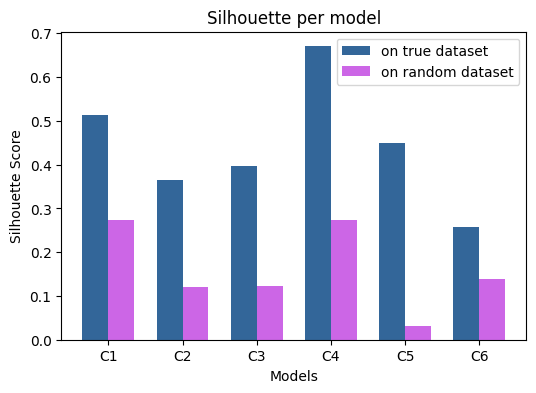
\includegraphics[width=.99\textwidth]{img/clustering/dbscan.png}
    \label{dbscan}
\end{figure}
\end{frame}

%%%%%%%%%%%%%%%%%%%%%%%%%%%%%%%%%%%%%%%%%%%%%%%%%%%%%%%%%%%%%%%%%%%%%%%%%%

\begin{frame}{Hierarchical Clustering}

    \begin{exampleblock}{Selected features:}
        \begin{itemize}
            \item latitude
            \item min\_age\_participants
            \item n\_killed
        \end{itemize}
    \end{exampleblock}

    
    
    \begin{table}[]
        \centering
        \begin{tabular}{|lc|}
            \hline  
            \textbf{Clustering}  & C4 \\
              \textbf{Best Method} & all\\
              \textbf{K} & 2\\
              \textbf{Clusters sizes} & (2088, 3938) \\
              \textbf{Silhouette} & 0.670266 \\
              \hline
        \end{tabular}
        \label{tab:my_label}
    \end{table}
\end{frame}

%%%%%%%%%%%%%%%%%%%%%%%%%%%%%%%%%%%%%%%%%%%%%%%%%%%%%%%%%%%%%%%%%%%%%%%%%%

\begin{frame}{Hierarchical Clustering}
    \begin{figure}
    \centering
    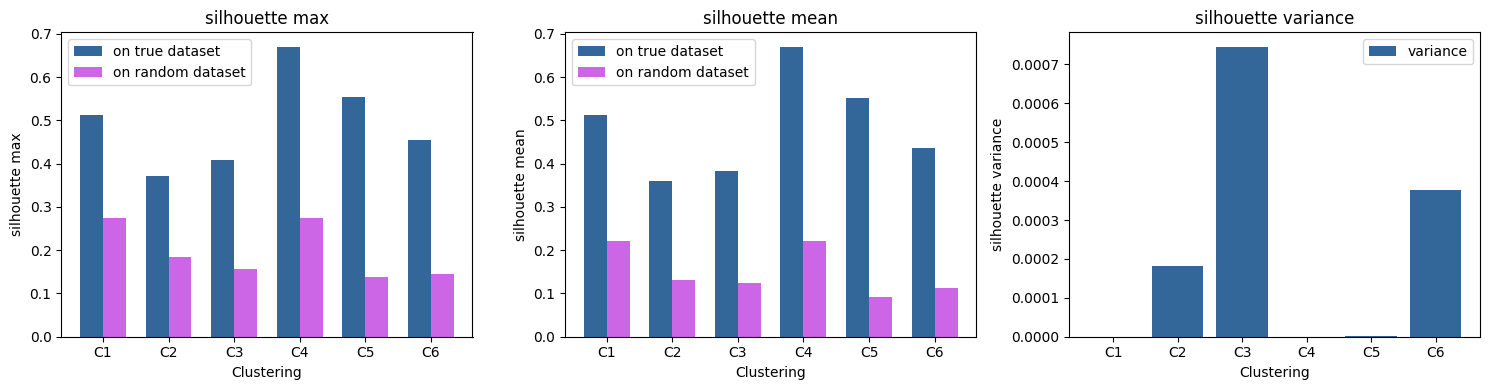
\includegraphics[width=.99\textwidth]{img/clustering/hier.png}
    \label{hier}
\end{figure}
\end{frame}

%%%%%%%%%%%%%%%%%%%%%%%%%%%%%%%%%%%%%%%%%%%%%%%%%%%%%%%%%%%%%%%%%%%%%%%%%%

\begin{frame}{DBSCAN and Hierarchical Clusters}
    \begin{figure}
    \centering
    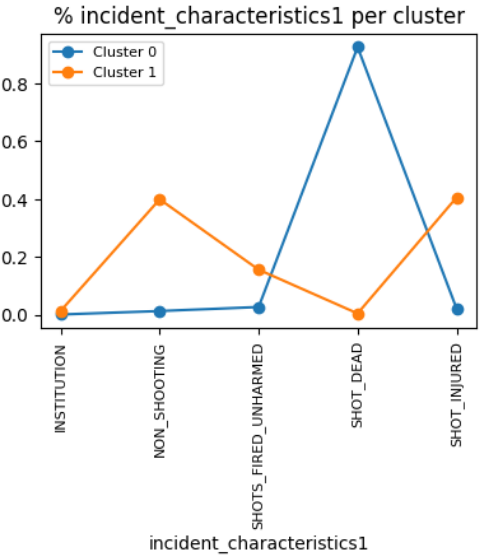
\includegraphics[scale=0.29]{img/clustering/dbscan1.png}
    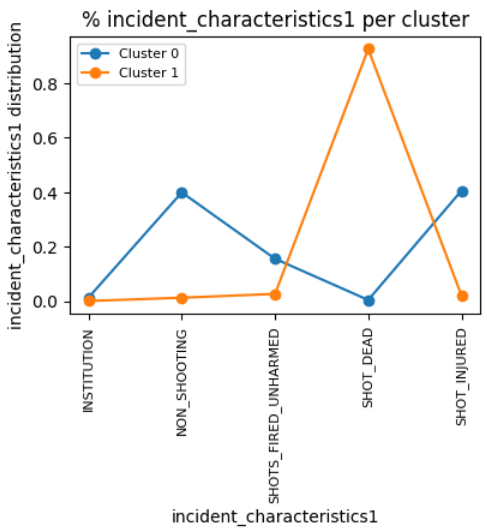
\includegraphics[scale=0.31]{img/clustering/hier2.png}
    \label{hier}
\end{figure}
\end{frame}

% \appendix

% \chapter{Questa è un'appendice}

\lipsum[5]

\section*{Questa è un'altra sezione, ma non viene inserita nell'indice}

\lipsum[6]


\bibliographystyle{plain}
\bibliography{chapters/Bibliografia.bib}


\end{document}
% -----------------------------------------------------------------
